\documentclass[10pt,journal,compsoc]{IEEEtran}

\usepackage[pdftex]{graphicx}    
\usepackage{cite}
\usepackage{subcaption} 
\hyphenation{op-tical net-works semi-conduc-tor}
\graphicspath{ {../images/} }

\begin{document}

\title{Robotics Software Engineer Nanodegree: Deep RL Arm Manipulation}
\author{Manuel Huertas L\'opez}

\markboth{Deep RL Arm Manipulation project, Robotic Nanodegree, Udacity}%
{}

\IEEEtitleabstractindextext{%

\begin{abstract}

Reinforcement learning is an area of ​​machine learning. It instructs an agent to take actions in an environment in order to maximize a cumulative reward. In this project a DQN algorithm will be used to guide a robotic arm to touch a cylindrical object. The idea behind the algorithm is to find an action value function; this function will give the cumulative expected reward for every state and action pair values. Once this function is obtained the action for every state will be the one that maximizes the reward. DQN is a variation of the algorithm where this function is replaced with a Deep Neural Network.

\end{abstract}

\begin{IEEEkeywords}
Robot, Udacity, Deep Reinforcemente Learning.
\end{IEEEkeywords}}

\maketitle
\IEEEdisplaynontitleabstractindextext
\IEEEpeerreviewmaketitle
\section{Introduction}

In this project a Robotic Arm with three degree of freedom will be taught in order to touch a cylindrical shape in the scene. Rather than using the forward and backward kinematic to calculate the position of the arm with respect to the joint angles or to move the arm to a goal position sending demands to the joints, the robot will try some random movements and it will receive a positive or negative reward. A video camera will be recording constatinualsy the robot movement and this information is used to train a neural network, the network will try to reproduce the sequence of movement that maximise the cumulative reward. As the final goal the robot will find the combination of joint movement, without a model, to approximate and finally touch the object in the scene.

Every Episodic finalized when the robot: touch the ground, touch the cylinder or the maximum number of iteration is reached. The final reward will be positive just in case the robot touch the cylinder, and there are some intermediate positive reward bases on smooth movement and when the robot is closer to the cylinder. The problem can be defined as a Markov Decision Process \cite{udacity} where:
\begin{itemize}
\item a finite set of states: the image from the video camera and all the pixel value combinations.
\item a finite set of actions: the movement every joint.
\item a finite set of rewards: the positive and negative reward depending on the robot behaviour.
\item the one-step dynamics of the environment: given the current state and the action, the expected new state and new reward. The neural network will obtain this during thetrainingg process.
\item a discount rate between [0,1]: the discount rate.
\end{itemize}

\label{sec:introduction}

\section{Background / Formulation}

Our goal is to find a function that for every state, the image in this case, tell use which action to take, the movement of the joint. This problem is not easy since there are a big number of states, pixel combination of the image, and sequences of movements. In this project an algorithm based in DQN have been used. In DQN a Deep Neural Network will build a function where the input will be the pixel of the image and the output the expected cumulative reward for every possible action. Selecting the action with the highest cumulative reward will give us the desired action. In addition, a Long Short Term Memory network have been used to use the information of the sequence of multiple images, instead of a single frame.

\subsection{Deep Q Network}

The Q-Learning algoritm is a model-free algoritm. The values for each state-action pair are estimated based on observation of the environment \cite{deepreinforcementlearning}. The Q-Learning algoritm estimate the state action funcition using the following equation:

\begin{align}
Q(s_{t},a_{t})=(1-\alpha) \cdot Q(s_{t},a_{t})+\alpha \cdot (r_{t}+\gamma max_a\cdot Q(s_{t+1},a))
\end{align}

The meaning of this parameter are:

\begin{itemize}
\item s: state value at time t, from the observation.
\item a: action value a time t.
\item alpha: learning rate, the way in which new values replaces old ones.
\item r: reward at time t.
\item gamma: discount factor.
\end{itemize}

In addition, the greedy policy is used to select between a current best action, exploit, or to select a random action, explore. If during the learning process we always select the action with currently the best reward we are never going to explore new solutions whose can give a better discounted future reward. On the other one, we need to select the current best action in order to use the knowledge we are acquiring iteratively. One way to accomplish this is to explore more at the beginning of the learning process, and gradually reduce the exploration favouring the exploitation of the current knowledge. For doing this the following parameters are defined:

\begin{itemize}
\item EPS\_START: starging gready value.
\item EPS\_END: ending gready value.
\item EPS\_DECAY: gready decay rate
\end{itemize}

Finally, the state action function is replaced with a deep neural network. The input of the network is the image from the video camera, and the output the reward or every action. The loss function, for the gradient descent algorithm, is defined as:

\begin{align}
Loss=1/2 \cdot [r_{t} + max_{a_{t+1}}\cdot Q(s_{t+a},a_{t+1};\theta_{t-1}}) - Q(s,a;\theta}]^2
\end{align}

Two extra techniques are included to make the neural network converge to the final solution. Experience replay, where a memory of experience is used to store previous values; mini-batches of these values are used as input of the neural network during learning. This technique helps to break the temporal dependencies of the learning process. Since the target of the loss function and the predictions have parameters in common, the process of learning can not converge to the correct solution, fixed Q targets is used to update the Q function after several iterations, in this way the small changes in the Q function approximation are not affecting the learning process.

The following extra parameters are defined.

\begin{itemize}
\item  INPUT\_WIDTH: Image from the camera, width
\item  INPUT\_HEIGHT: Image from the camera, height
\item  OPTIMIZER: Optimizer for the gradient descent algorithm 
\item  LEARNING\_RATE: Neural Network learning rate.
\item  REPLAY\_MEMORY: Size of the memory for the experience replay technique.
\item  BATCH\_SIZE: Batch size for the experience replay technique.
\end{itemize}

\subsection{Long Short Term Memory}

LSTM is a special Recurrent Neural Network, capable of learning long-term dependencies. The Long short-term memory adds memory to the DQN to remember the sequence of movements of the joint to find and touch the object in the scene \cite{lstmnetwork}.

\section{Robotic Arm}

In a reinforcement learning problem, a temporary series of interactions are produced until the episodic ends: S_{0},A_{0},R_{1},S_{1},A_{1},R_{2},...,R_{T},S_{T}

In this project, an episode ends when: the robot's arm touches the ground, a maximum of iterations is reached, or the robot touches the object in the scene; the states are the image, captured by the video camera, of the scene; the actions can be to move the joints at random using position or speed control; finally, the reward strategy is defined as a negative number when the robot finishes the episodic without touching the object, the positive number when it touches the object and an incremental or decremental reward when the arm approaches the target or not.

Different reward strategies were tested, the final choose solution was: a big number positive number when the robot touches the object; a negative number when the robot touch the ground or the maximum iterations are reached, to this negative number a 1\% of the distance to the goal is added, in order to decrease the negative reward depending on the closest to the goal; a smooth reward when the robot is searching the object in function of the smoothest of the movement and the distance to the goal.

\subsection{Rewards}

The positive reward when the object is touched is 1000000.0. The negative base reward is -1.0. When the episodice ends without success to the negative base reward is added 1\% the distance to the goal. Finally when the Robot is searching a soomoth average goal delta is added to the distance to the goal as follow:

AverageGoalDelta  = ( AverageGoalDelta * 0.2 ) + (DistanceDelta * (1-0.2));

Reward Searching  = AverageGoalDelta + 0.01*exp(-pow(DistanceGoal,2));

The same rewards were used for both objectives. 

\subsection{Hiper Paramters}

Finally the hiper-parameters selecting were:

\begin{itemize}
\item  VELOCITY\_CONTROL[false]: The position control was used.
\item  NUMBER\_ACTIONS[6]: The number of actions was calculated as number of DOF x 2.
\item  ALLOW\_RANDOM[true]: The learnning process allows random decisions to explore new solutions.
\item  GAMMA[0.9]: discount factor, selected was 0.9.
\item  EPS\_START[0.9]: Starting greedy value.
\item  EPS\_END[0.01] Ending greedy value.
\item  EPS\_DECAY[200]: Greedy decay rate
\item  INPUT\_WIDTH[64]: Image from the camera width
\item  INPUT\_HEIGHT[64]: Image from the camera height
\item  OPTIMIZER[RMSprop]: Optimizer for the gradient descent algorithm 
\item  LEARNING\_RATE[0.01]: Neural Network learning rate.
\item  REPLAY\_MEMORY[10000]: Size of the memory for the experience replay technique.
\item  BATCH\_SIZE[64]: Batch size for the experience replay technique.
\item  USE\_LSTM[true]: Uses Long Short Memory.
\item  LSTM\_SIZE[512]: Sizes of the LSTM network.
\end{itemize}

The same Hiper Parameters were used for both objectives. 

\section{Results}

In order to find the reward and hiper-parameters a trial and error strategy was used. At the beginning velocity control was used, but the desired accuracy of 80\% of success touching the object with the gripper base was not achieve, for that reason the position control was selected. The reward strategy consists in give a high positive number when the robot touches the object, this big number was selected because the robot could accumulate small rewards during the searching process and it was important to stimulate the robot not to keep searching but to move toward the goal. During the searching process a small amount of the distance to goal was added to the reward to indicate the robot's arm that the action should move the arm in the object direction. Also, a factor depending on of the delta movement, was used to increase, when the movement was directing the robot to the goal, or decrease when the movement was in the other direction. This searching strategy was used to indicate the robot's arm to keep moving and to do it smoothly  to the goal direction. Finally, when the robot ends the episodic without success, a negative reward is given. To this negative reward a factor of the distance to the goal is added to indicate the robot how close was to the solution, even having failed.

\begin{figure}[h]
\centering
\begin{subfigure}[b]{0.4\textwidth}
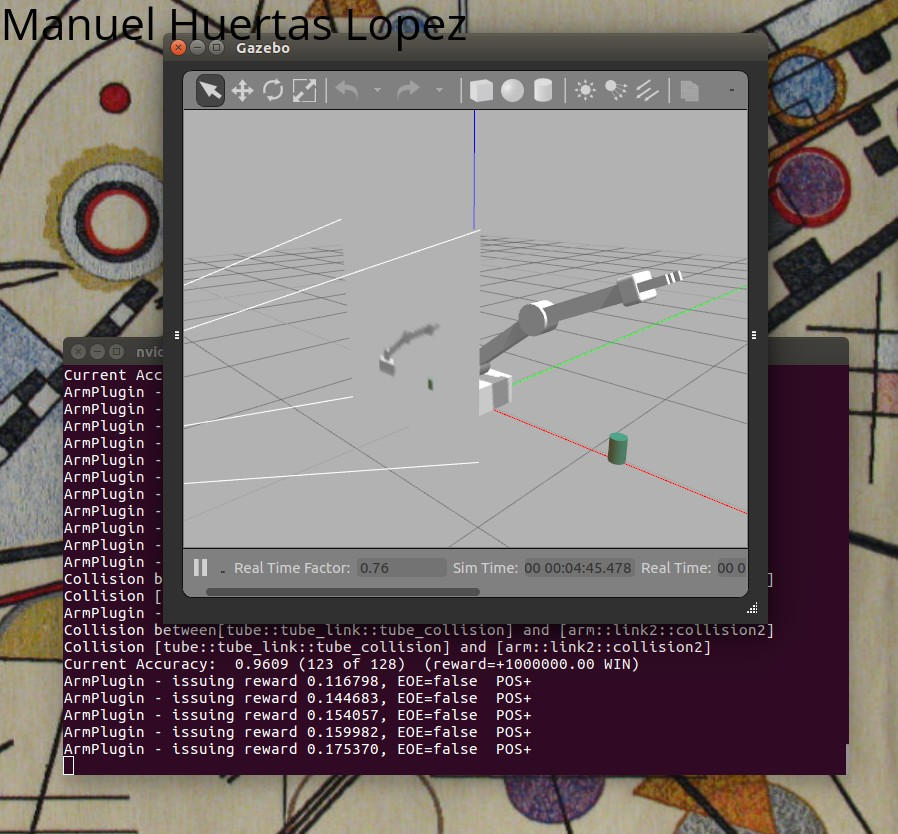
\includegraphics[scale=0.25]{Learnning_Collision_ARM}
\caption{Robot's Arm touching the object}
\end{subfigure}
\begin{subfigure}[b]{0.4\textwidth}
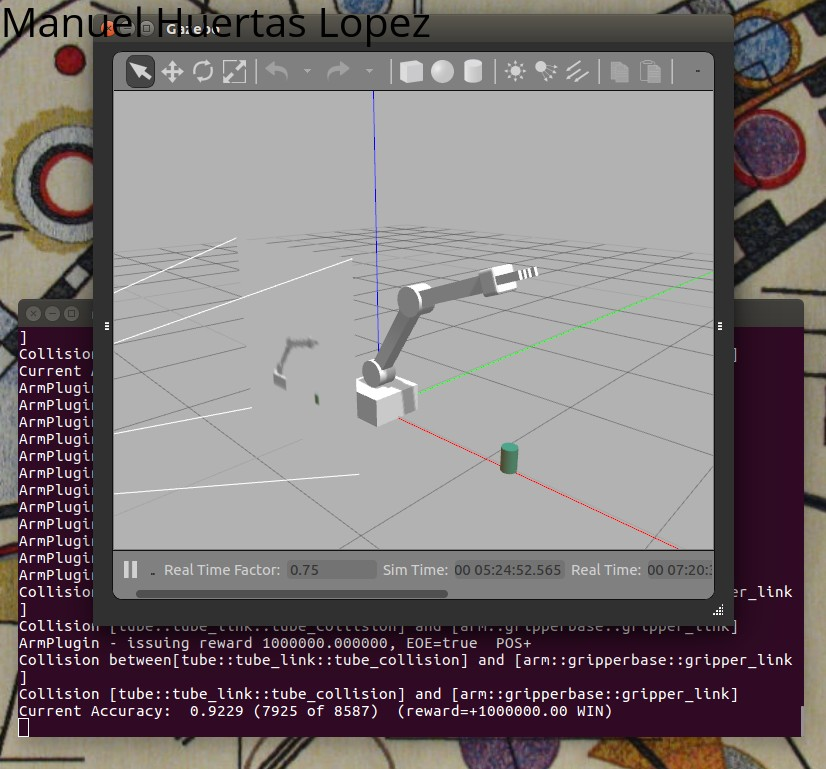
\includegraphics[scale=0.27]{Learnning_Collision_Gripper}
\caption{Robot's Arm touching the object with the base gripper}
\end{subfigure}
\caption{Robot's Arm}
\end{figure}

\section{Discussion}

The project consists in completing eight tasks:

\begin{enumerate}
\item  Subscribe to camera and collision topics: This was easily achieved following the udacity instructions.
\item  Create the DQN Agent: Udacity provided the class, it was just necessary to create an instance.
\item  Velocity or position based control of arm joints: position control was selected because it was easier to define the rewards.
\item Reward for robot gripper hitting the ground: using a bounding box for the gripper it was detected when it was hitting the ground; a negative reward plus a 1\% to the distance to the goal was used.
\item Issue an interim reward based on the distance to the object: an incremental, reward positive or negative, was used, depending on the robot movement to the goal or not.
\item Issue a reward based on collision between the arm and the object: a very high number was used to stimulate the robot to move to the goal.
\item Tuning the hyper parameters: a trail an error approach was used to find the final parameters.
\item  Issue a reward based on collision between the arm’s gripper base and the object: the same reward and hyper parameters were used for the two objectives.
\end{itemize}


\section{Conclusion / Future work}

In order to improve the project a deeper understating about how the reward affects the learning process will be needed. A way to do this can be to visualize the Q-Function using a 2D plot where the x-axis can be the actions, y-axis the state, and the coloured value of the graph the reward. The rewards were selected using some logic about how the human will learn to solve the problem. Different strategies will be needed to be explored in order to find a solution that converges quicklier to the final solution.

% Bibliography
\begin{thebibliography}{9}
\bibliographystyle{ieeetr}

\bibitem{udacity} 
Robotics Software Engineer Nanodegree program
\textit{https://eu.udacity.com}

\bibitem{deepreinforcementlearning} 
\textit{Human-level control through deep reinforcement learning}. 

\bibitem{lstmnetwork} 
Understanding LSTM Networks
\textit{http://colah.github.io/posts/2015-08-Understanding-LSTMs}

\end{thebibliography}

\end{document}